\documentclass[a4paper ,12pt, onecolumn]{article}
\usepackage[utf8]{inputenc}
\usepackage[spanish]{babel}
\usepackage[hidelinks]{hyperref}
\usepackage{graphicx}
\begin{document}
\title{Anexo diseño mecánico}

\author{Rubén Arce}
\date{\today}
\maketitle
\cleardoublepage
\tableofcontents
\listoffigures
\cleardoublepage

\section{Introducción}
Para llevar a cabo el diseño mecánico de estas piezas concretas se ha optado por emplear Freecad, un
programa de software libre que permite hacer modelos sencillos de forma gratuita.
Se ha empleado la versión 12 del mismo corriendo en una raspberry pi 4 de 4Gb de RAM, este es el único
programa que corre en linux de diseño 3D y además consume pocos recursos.
\paragraph{}
Los primeros prototipos se han llevado a cabo con una impresora 3D Anet A8 con el firmware de Marling
2.0 y como material PLA de 1,75mm y distancia entre capa de 0,2 mm.
\section{Emisor beacon}
    \subsection{Aspectos a considerar en el diseño}
        \begin{enumerate}
            \item Estéticamente atractivo
            \item Pequeñas dimensiones
            \item Cómodo para llevar colgado del cuello
            \item Facilidad para desmontar y recargar las baterías o pilas
            \item Limitaciones en el tamaño de máximo 220x220x250 mm debido al volumen de impresión.
        \end{enumerate}
    \subsection{Planos y dimensiones}
        Una vez llevado a cabo el siseño se han obtenido los planos y se ha llevado a cabo la impresión 3d de los mismos.
        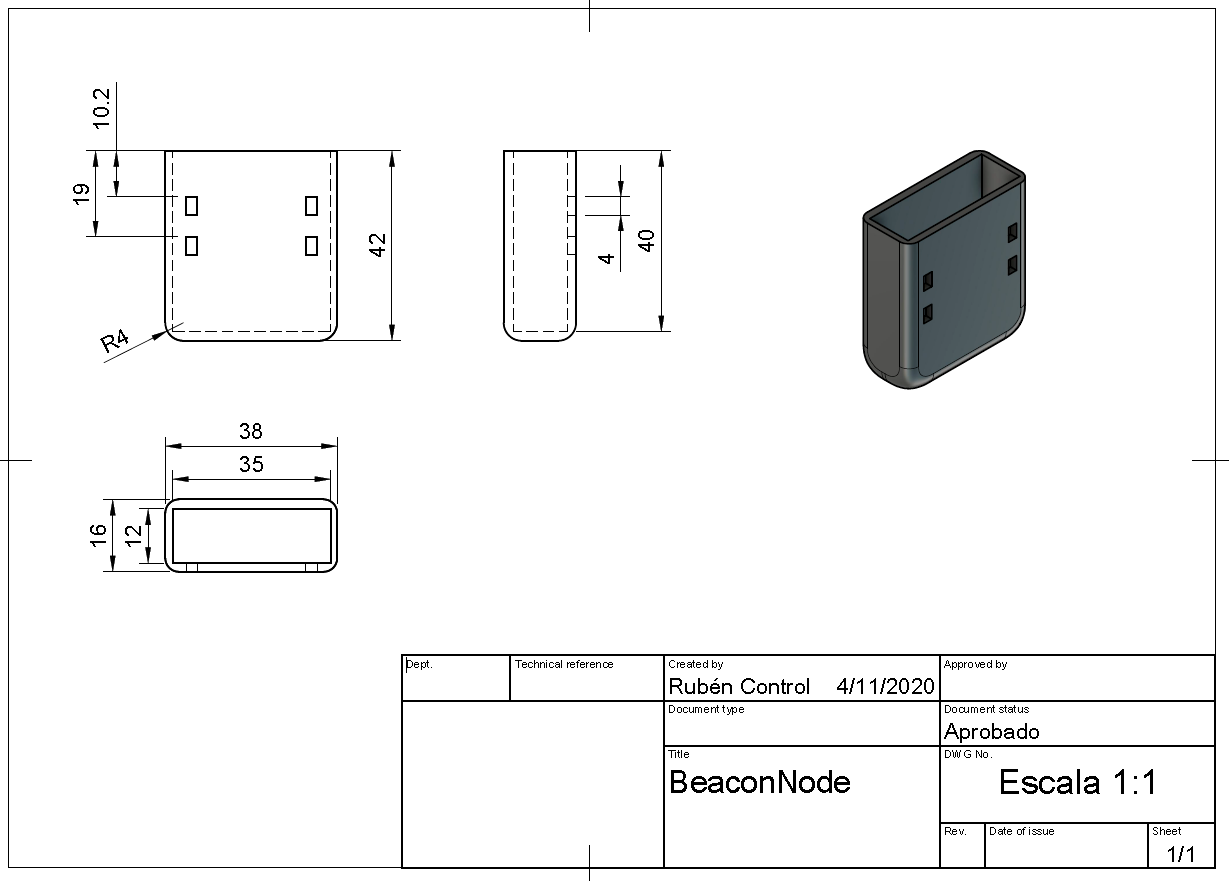
\includegraphics[scale=0.25]{../model_beacon.PNG}
    \subsection{Imágenes renderizado}
    \begin{center}
        \begin{center}
            \begin{figure}[h]
                \centering
                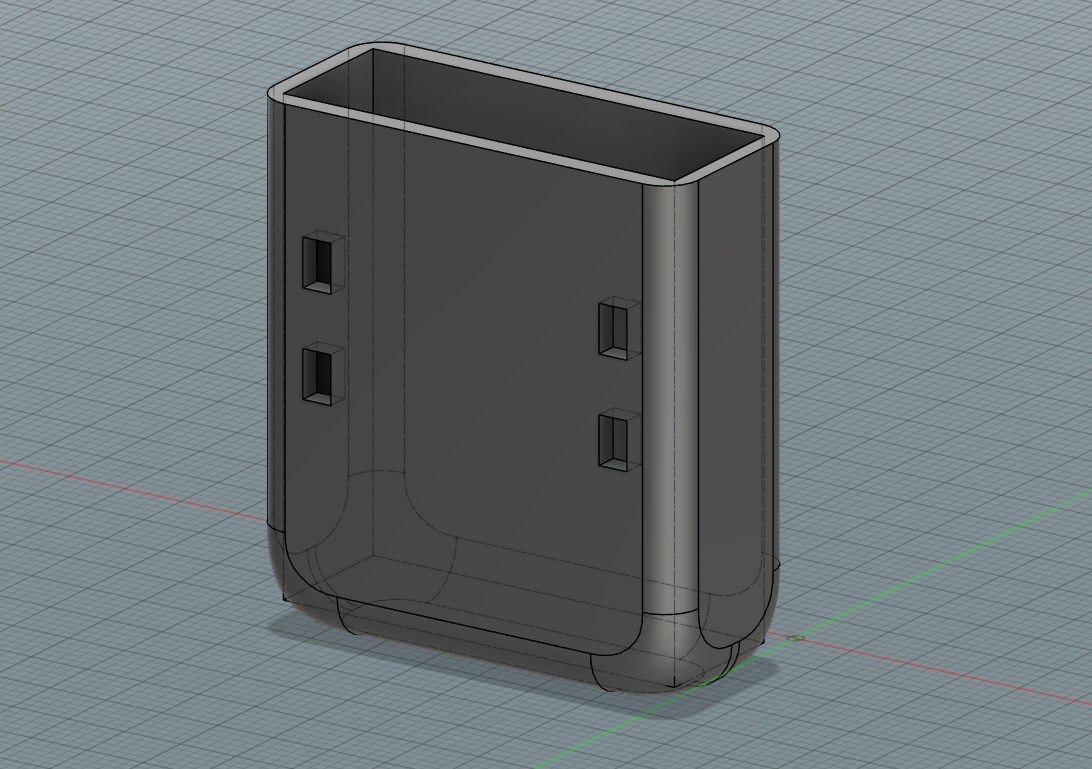
\includegraphics[width=0.3\textwidth]{../mechanical_beacon.PNG}
                \caption{Prototipo impreso con Anet A8 master v1}
                \label{fig:mesh1}
            \end{figure}
        \end{center}
        \begin{center}
            \begin{figure}[h]
                \centering
                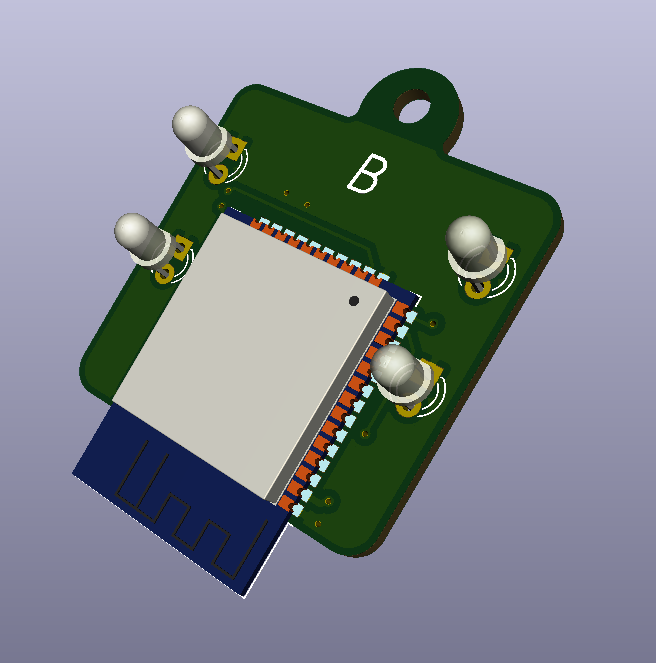
\includegraphics[width=0.3\textwidth]{../emiter_1.PNG}
                \caption{Prototipo impreso con Anet A8 master v1}
                \label{fig:mesh1}
            \end{figure}
        \end{center}
    \end{center}
    \subsection{Imágenes reales}

        \begin{center}
            \begin{figure}[h]
                \centering
                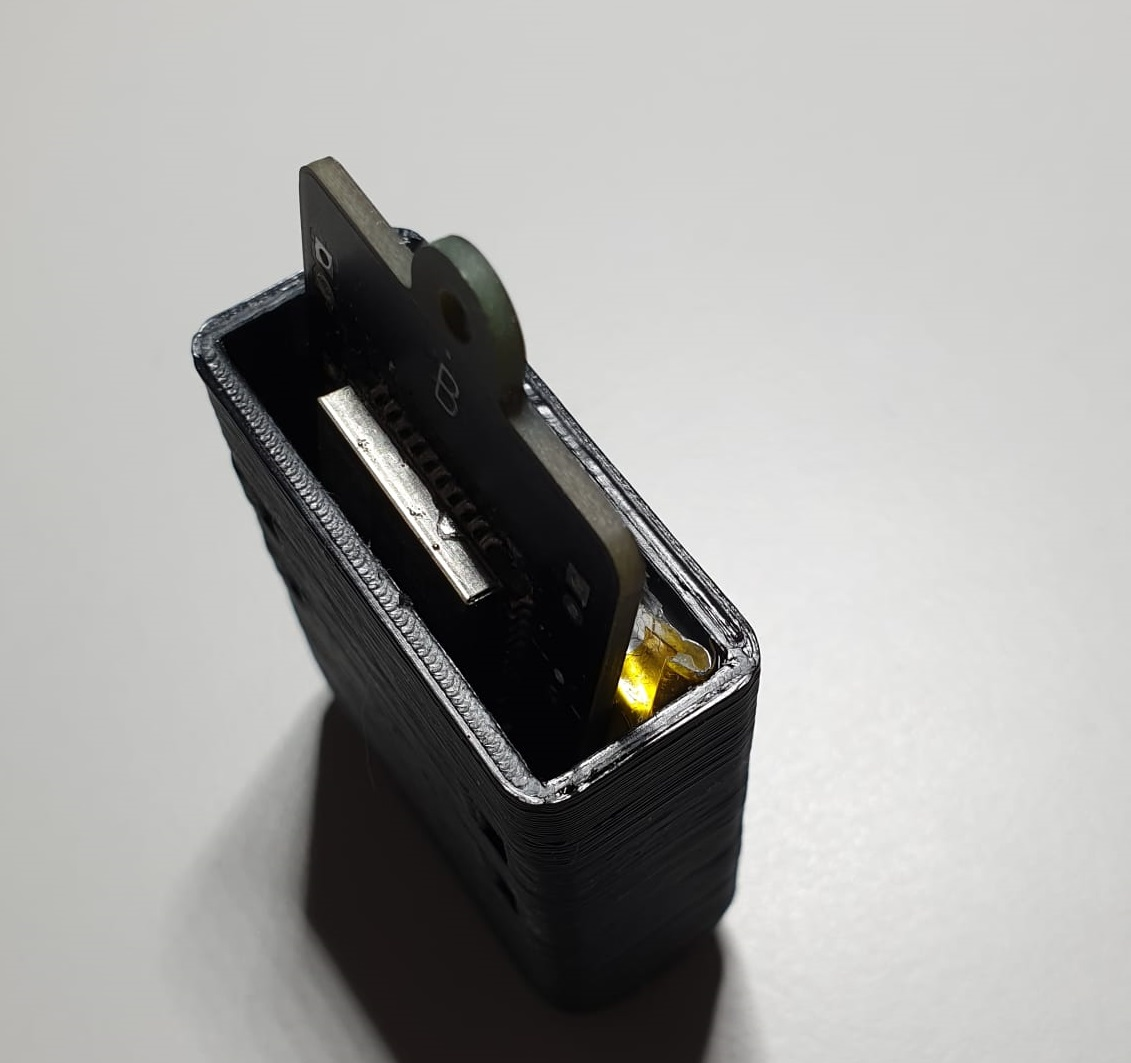
\includegraphics[width=0.3\textwidth]{../3d_beacon_1.jpeg}
                \caption{Prototipo impreso con Anet A8 master v1}
                \label{fig:mesh1}
            \end{figure}
        \end{center}
        \begin{center}
            \begin{figure}[h]
                \centering
                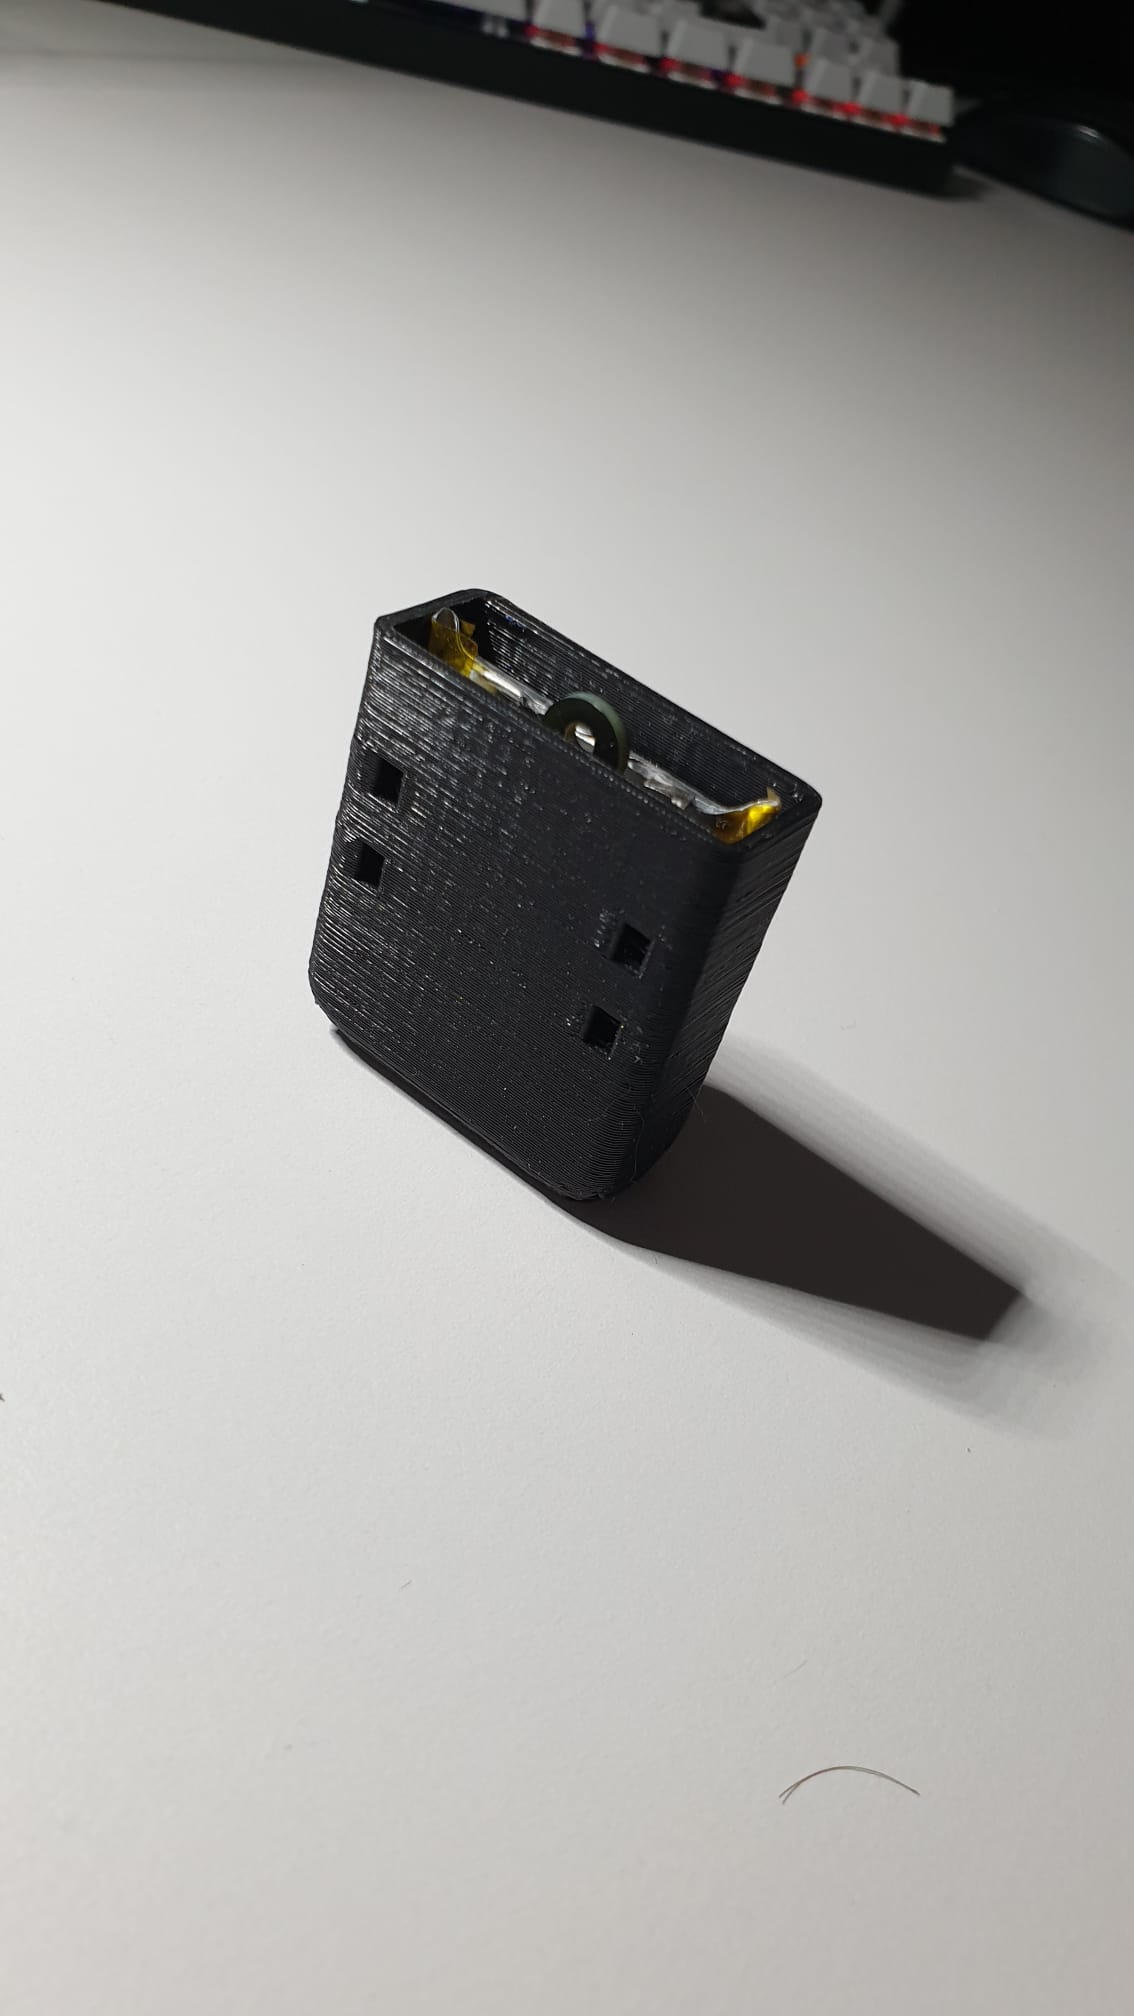
\includegraphics[width=0.3\textwidth]{../3d_beacon_2.jpeg}
                \caption{Prototipo impreso con Anet A8 master v1}
                \label{fig:mesh1}
            \end{figure}
        \end{center}

\section{Receptor beacon o gateway}
    \subsection{Aspectos a considerar en el diseño}
        \begin{enumerate}
            \item Estéticamente atractivo, puesto que va a estar físicamente a la vista.
            \item Pequeñas dimensiones y discreto.
            \item Limitaciones en el tamaño de máximo 220x220x250 mm debido al volumen de impresión.
            \item Estructura sólida que garantize un buen agarre de la PCB en vertical.
        \end{enumerate}
    \subsection{Planos y dimensiones}
        Partiendo de las dimensiones de la tarjeta que se muestra a continuación:
        \begin{center}
            \begin{figure}[h]
                \centering
                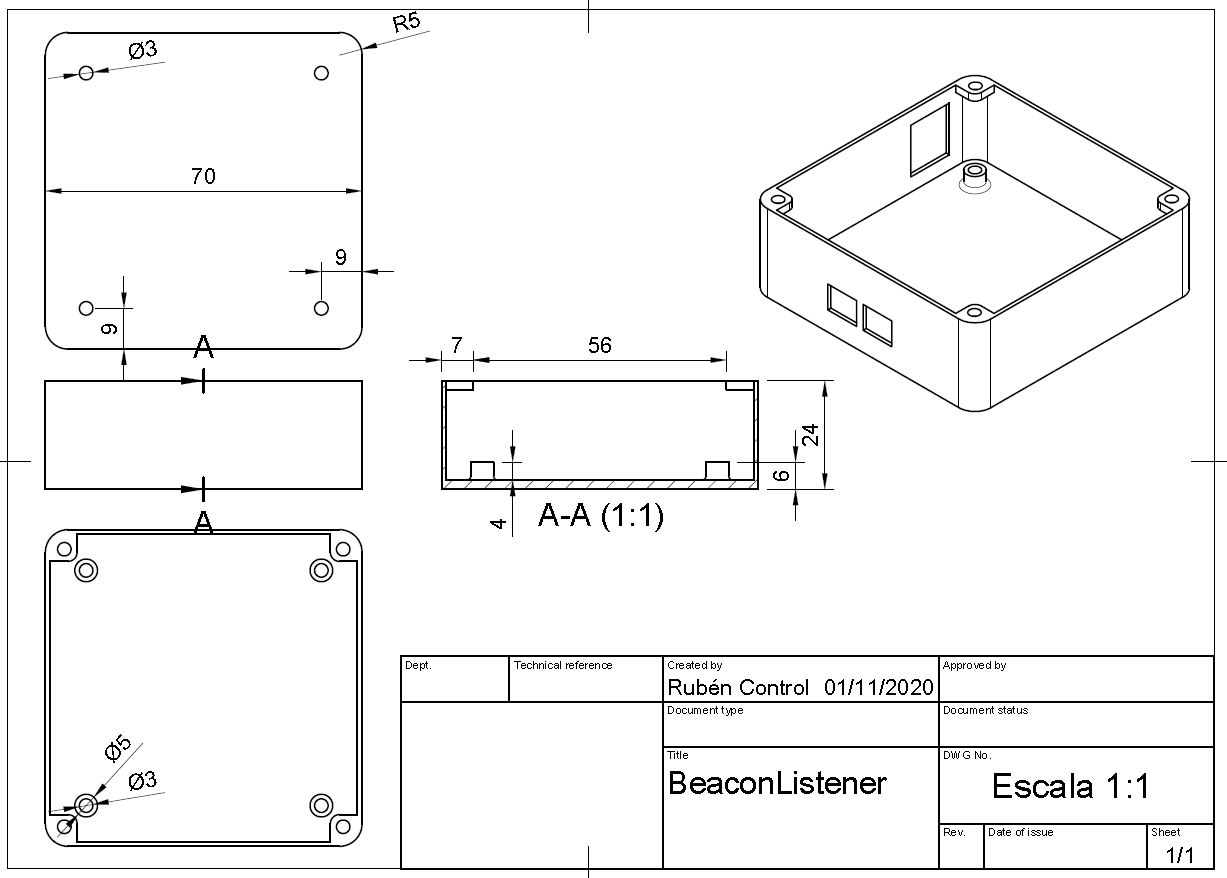
\includegraphics[width=0.55\textwidth]{../model_master.PNG}
                \caption{Plano caja del emisor}
                \label{fig:mesh1}
            \end{figure}
        \end{center}

        Se ha prototipado el siguiente diseño:
    \subsection{Imágenes renderizado}


        Los renderizados 3D previos a la impresión:
        \begin{center}
            \begin{figure}[h]
                \centering
                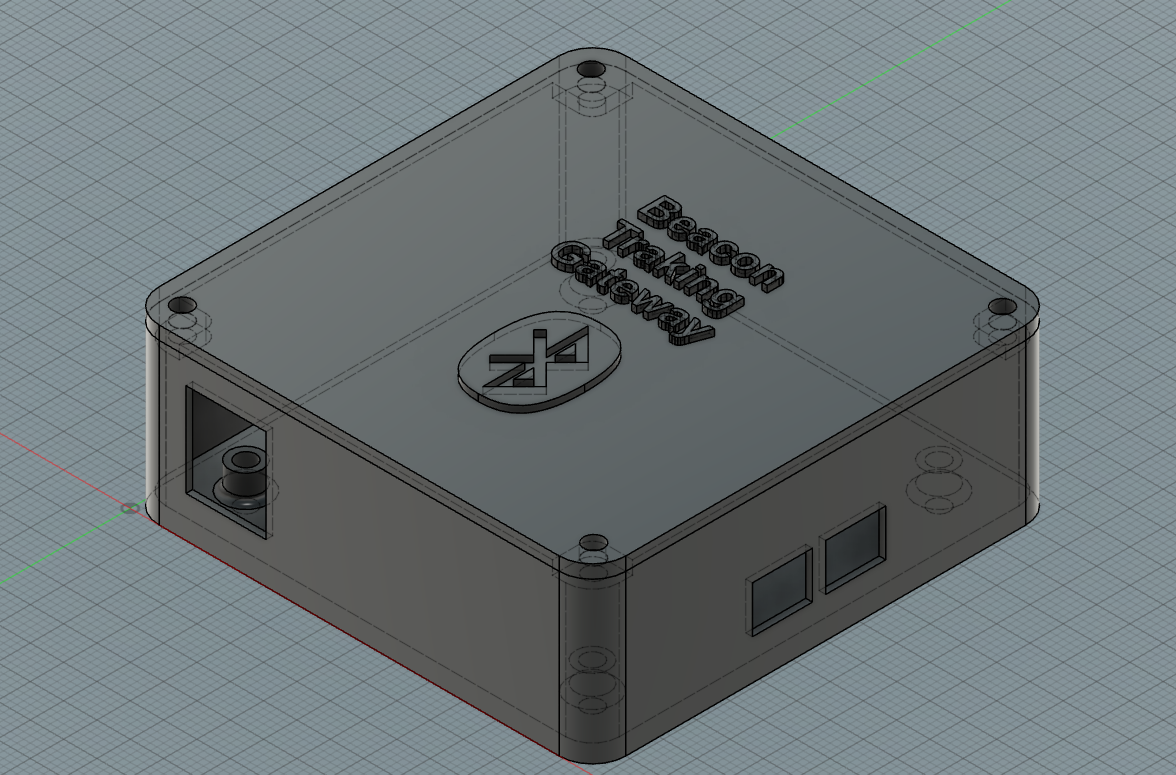
\includegraphics[width=0.55\textwidth]{../mechanical_master.PNG}
                \caption{Renderizado caja del emisor}
                \label{fig:mesh1}
            \end{figure}
        \end{center}
        \begin{center}
            \begin{figure}[h]
                \centering
                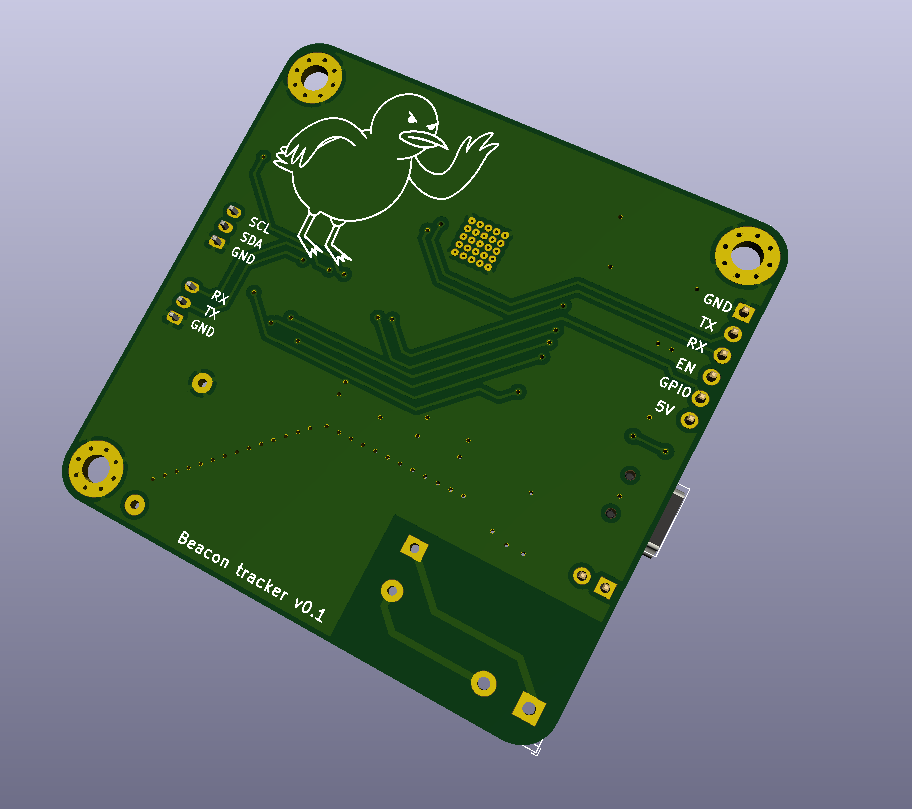
\includegraphics[width=0.55\textwidth]{../receiver_2.PNG}
                \caption{Plano caja del emisor}
                \label{fig:mesh1}
            \end{figure}
        \end{center}

    \subsection{Imágenes reales}
        Una vez impresas las piezas y sin necesidad de lijar o ajustar algún apriete o tolerancia:
    
        \begin{center}
            \begin{figure}[h]
                \centering
                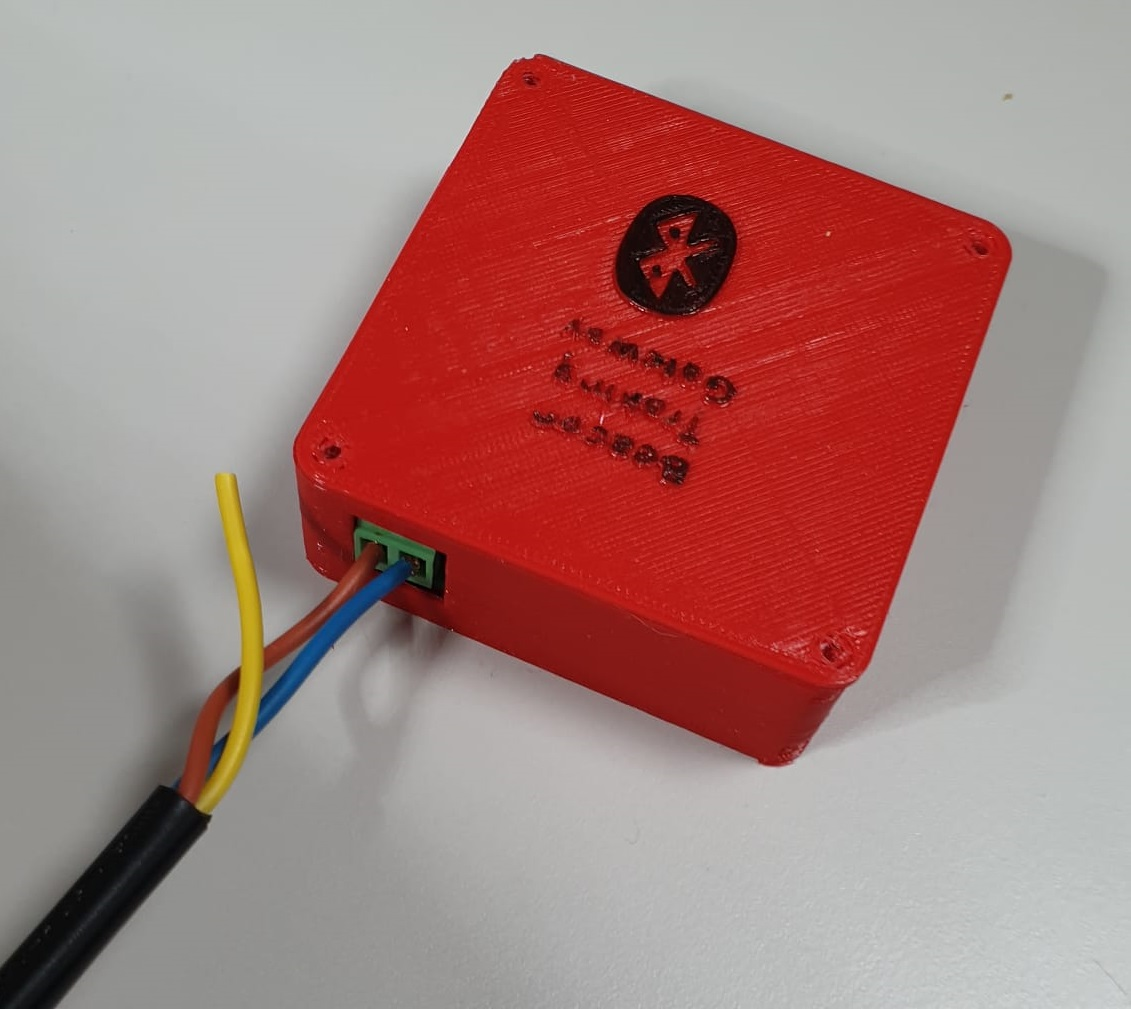
\includegraphics[width=0.3\textwidth]{../3d_master_1.jpeg}
                \caption{Prototipo impreso con Anet A8 master v1}
                \label{fig:mesh1}
            \end{figure}
        \end{center}
        \begin{center}
            \begin{figure}[h]
               \centering
                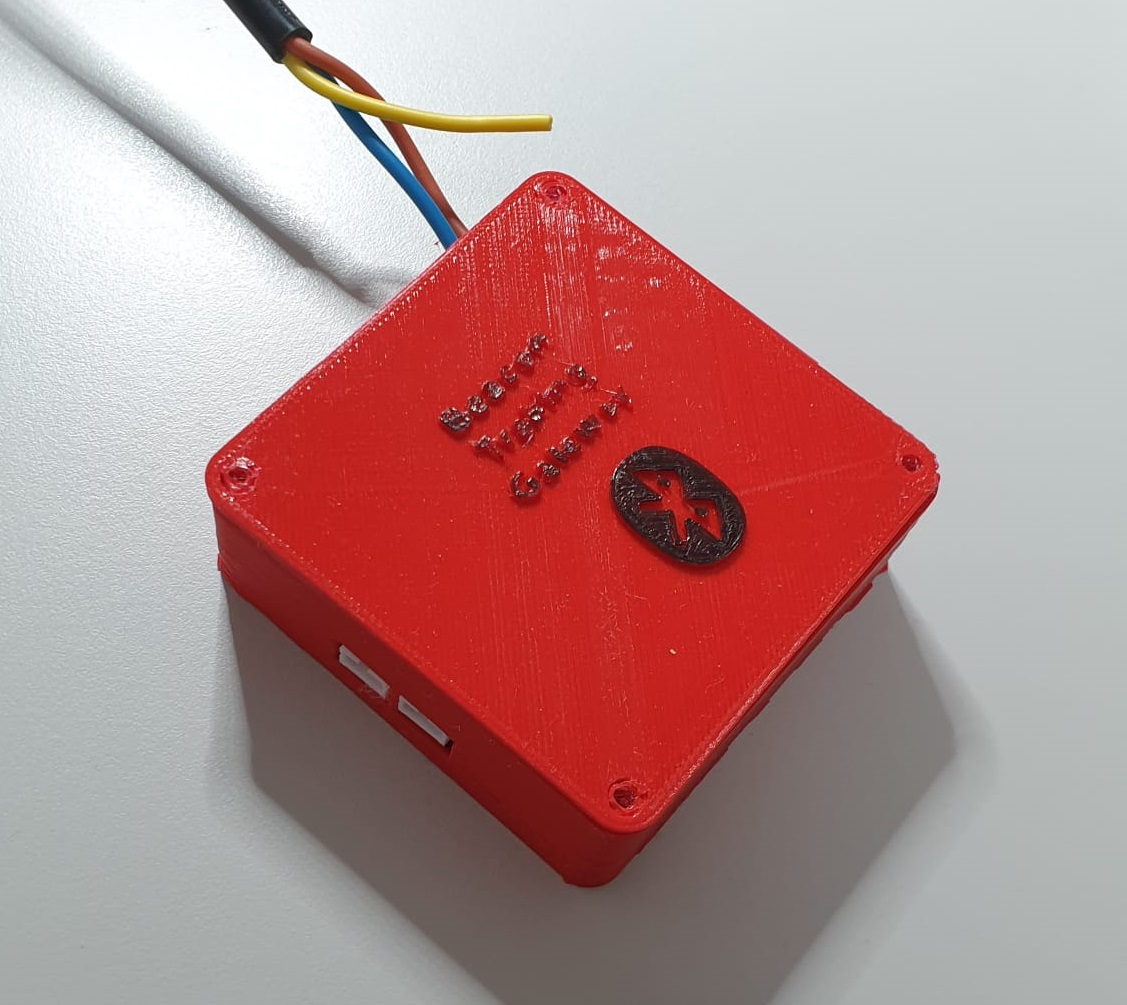
\includegraphics[width=0.3\textwidth]{../3d_master_2.jpeg}
                \caption{Prototipo impreso con Anet A8 master v2}
                \label{fig:mesh1}
            \end{figure}
        \end{center}

\section{Conclusiones}
    Tras desarrollar los primeros prototipos se procedió a llevar a cabo una prueba real con los mismos 
    en un entorno industrial para comprobar si era necesaria una versión 2.0 de los mismos, los resultados
    dejaron claro que este primer diseño era el acertado.

    Execeptuando una caida accidental todos los diseños sobrevivieron a la prueba, las imágenes dentro de la planta
    no han sido posibles de llevar a cabo por seguridad y ausencia de permisos por parte de administración.

\end{document}